\documentclass[]{beamer}
\usepackage[utf8]{inputenc}
\usepackage[T1]{fontenc}
\usepackage{carlito}
\usetheme[horizontal=true, hr=false, pagenumbers=true]{NewPwr}
\usepackage{bibentry}
\usepackage{minted}
\setminted{fontsize=\small,baselinestretch=1}
\usepackage{multicol}
\usepackage{polski}
\usepackage{setspace}

% Build-specific command
\nonstopmode

%Information to be included in the title page:
\title{Opracowanie algorytmu generacji grafu DSP do rozwiązania problemu syntezy dźwięku}
\subtitle{Design of a DSP graph generation algorithm for solving the sound synthesis problem}
\author{Autor pracy: Mateusz Bączek \\ Opiekun pracy: Dr Inż. Maciej Hojda}
\institute{Seminarium Dyplomowe -- prezentacja 1}
\date{2023}

\begin{document}
\onehalfspacing
\frame{\titlepage}

\section{Wstęp teoretyczny}

% \begin{frame}
% \frametitle{Definicja problemu}
% % \vspace{-1cm}
%   \begin{enumerate}
%     \item Tworzymy produkt,
%     \item uruchamiamy produkt (na sprzęcie dedykowanym/w chmurze/na sprzęcie klienta),
%     \item \textbf{czy produkt \textit{działa}?}
%   \end{enumerate}
% \end{frame}

\begin{frame}
  \frametitle{Kompozycja algorytmiczna}

  \begin{multicols}{2}
  \begin{figure}
    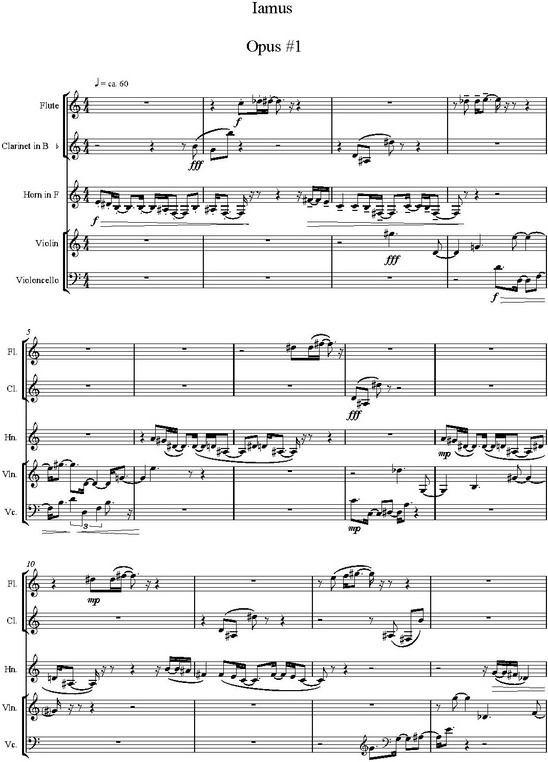
\includegraphics[width=0.7\linewidth]{lamus_notes.jpg}
    \caption{Zapis nutowy utworu wygenerowany przez komputer \textit{Lamus}.}
  \end{figure}

  \begin{figure}
    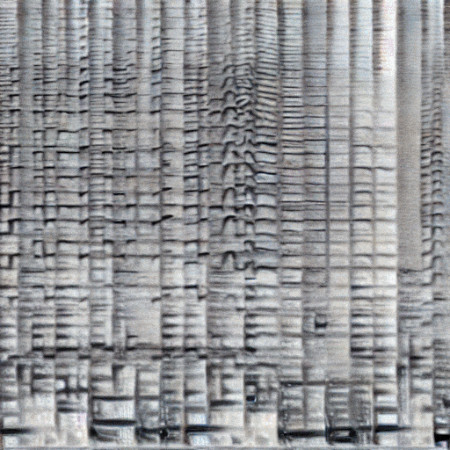
\includegraphics[width=0.8\linewidth]{riffusion_spectro.jpg}
    \caption{Spektrogram wygenerowany przez algorytm \textit{Stable Riffusion}.}
  \end{figure}
  \end{multicols}

\end{frame}


\begin{frame}
  \frametitle{Rozpowszechnione podejścia do kompozycji komputerowej}

  \begin{enumerate}
    \item Generowanie zapisu nutowego \cite{language_models_drummers}:
      \begin{itemize}
        \item wykorzystuje reguły matematyczne oparte o teorię muzyki,
        \item generuje zapis symboliczny, który łatwo później wykorzystać.
      \end{itemize}
    \item Generowanie pełnego pliku audio \cite{riffusion}:
      \begin{itemize}
        \item teoretycznie najbardziej imponujący efekt działania,
        \item małe możliwości wykorzystania rezultatu algorytmu.
      \end{itemize}
    \item Generowanie brzmienia za pomocą sieci neuronowych \cite{nsynth}:
      \begin{itemize}
        \item potencjalnie bardzo szeroka gama generowanych brzmień,
        \item małe możliwości dostosowania brzmienia,
        \item słaby wgląd we ,,wnętrze'' wygenerowanego algorytmu DSP.
      \end{itemize}
  \end{enumerate}
\end{frame}

\begin{frame}
  \frametitle{Elementy kompozycji muzycznej}
  \begin{figure}[H]
    \centering\small
    \begin{center}
    \begin{tikzpicture}
      \begin{scope}[blend group = soft light]
        \fill[red!30!white]    ( 90:1.5) circle (1.7);
        \fill[blue!30!white]   (210:1.5) circle (1.7);
        \fill[orange!30!white] (330:1.5) circle (1.7);
      \end{scope}
      \node at (90: 1.5) [align=center] {\small Linia \\ melodyczna};
      \node at (210:1.5) [align=center] {\small Modulacja};
      \node at (330:1.5) [align=center] {\small Barwa \\ dźwięku};
      % \node[align=center] { \textbf{Wspólna} \\ \textbf{pętla zdarzeń} \\ \textbf{\texttt{asyncio}}};
    \end{tikzpicture}
    \end{center}
    \caption{
      Elementy opisujące pojedynczy głos/instrument w kompozycji muzycznej. 
    }
    \label{telemetry_backend_asyncio}
  \end{figure}
\end{frame}


\begin{frame}
  \frametitle{Cel pracy}

  \centering
  \Large
  Wytworzenie dźwieku o określonej \textbf{barwie}
\end{frame}


\begin{frame}
  \frametitle{Skąd bierze się \textbf{barwa} dźwięku?}
  \begin{figure}
    \centering
    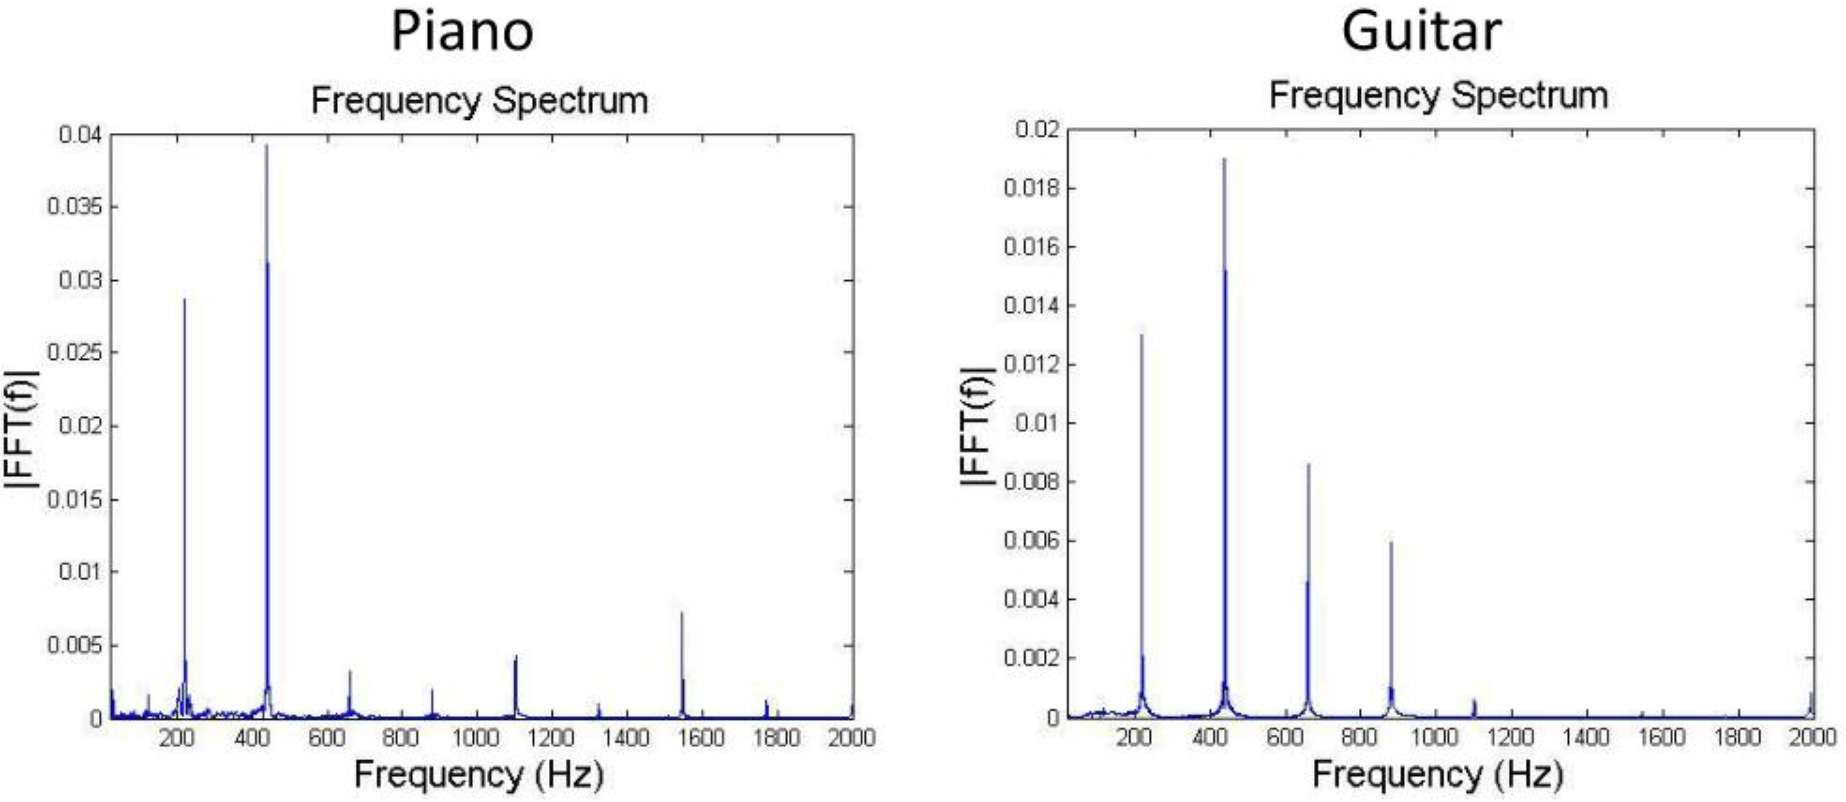
\includegraphics[width=0.9\linewidth]{piano_guitar_fourier.png}
    \caption{Porównanie transformaty Fouriera dla dźwięku pianina i gitary na tej samej wysokości.}
  \end{figure}
\end{frame}


\begin{frame}
  \frametitle{Jak kontroluje się barwę w syntezatorach dźwięku}

  \begin{figure}
    \centering
    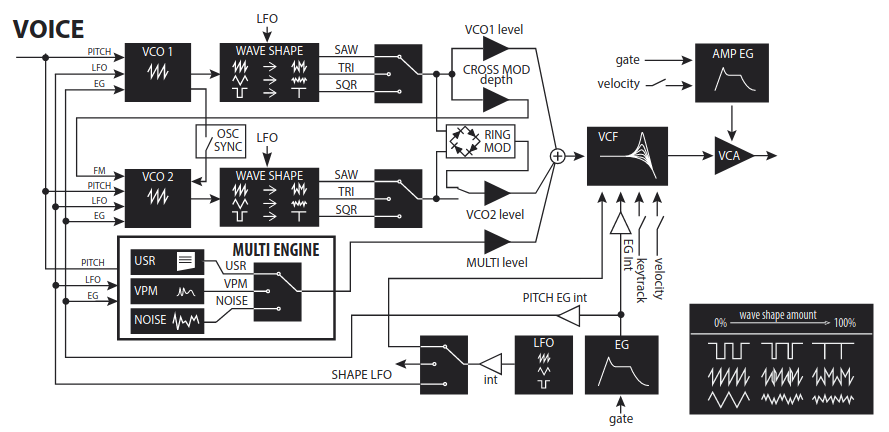
\includegraphics[width=0.9\linewidth]{minilogue_voice_block_diagram.png}

    \caption{
      Diagram blokowy pojedynczego głosu w syntezatorze 
      \textit{Minilogue xd} \cite{minilogue_diagram}.
    }
  \end{figure}
\end{frame}


\begin{frame}
  \frametitle{Generalizacja tradycyjnego procesu syntezy dźwięku}

  \begin{enumerate}
    \item Bloki generujące sygnał:
      \begin{enumerate}
        \item synteza prostych sygnałów (sinus, trójkąt, prostokątny),
        \item odtwarzanie sampli dźwiękowych,
        \item sygnał modulujący (rytm, \textit{ADSR}).
      \end{enumerate}
    \item Bloki przetwarzające sygnał:
      \begin{enumerate}
        \item filtry (górnoprzepustowy, dolnoprzepustowy, itd.),
        \item efekty (pogłos, echo).
      \end{enumerate}
    \item Połączenia między blokami:
      \begin{enumerate}
        \item modulowanie parametrów bloku przetwarzania sygnału.
      \end{enumerate}
  \end{enumerate}
\end{frame}

\begin{frame}
  \begin{multicols}{2}
  \begin{figure}
    \centering
    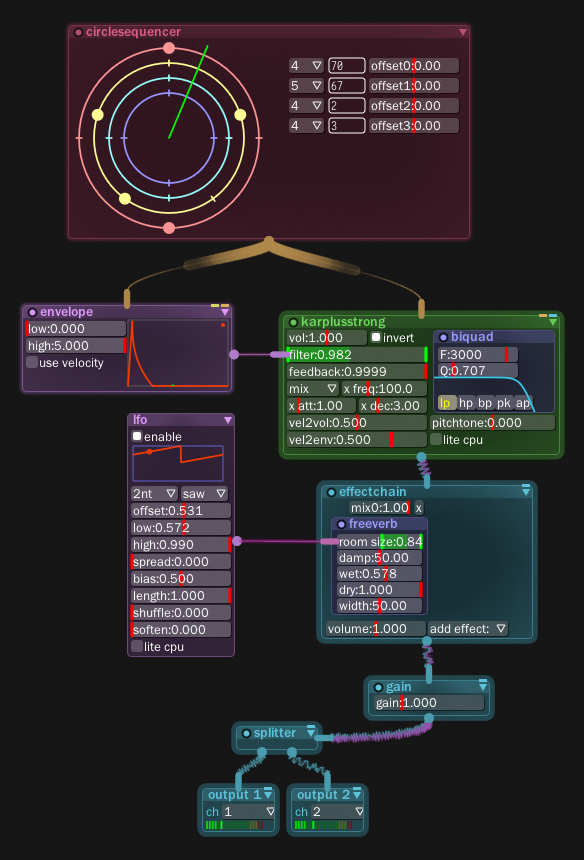
\includegraphics[width=1.0\linewidth]{bespoke.png}
    \caption{Oprogamowanie \textit{Bespoke Synth}.}
  \end{figure}

  \begin{figure}
    \centering
    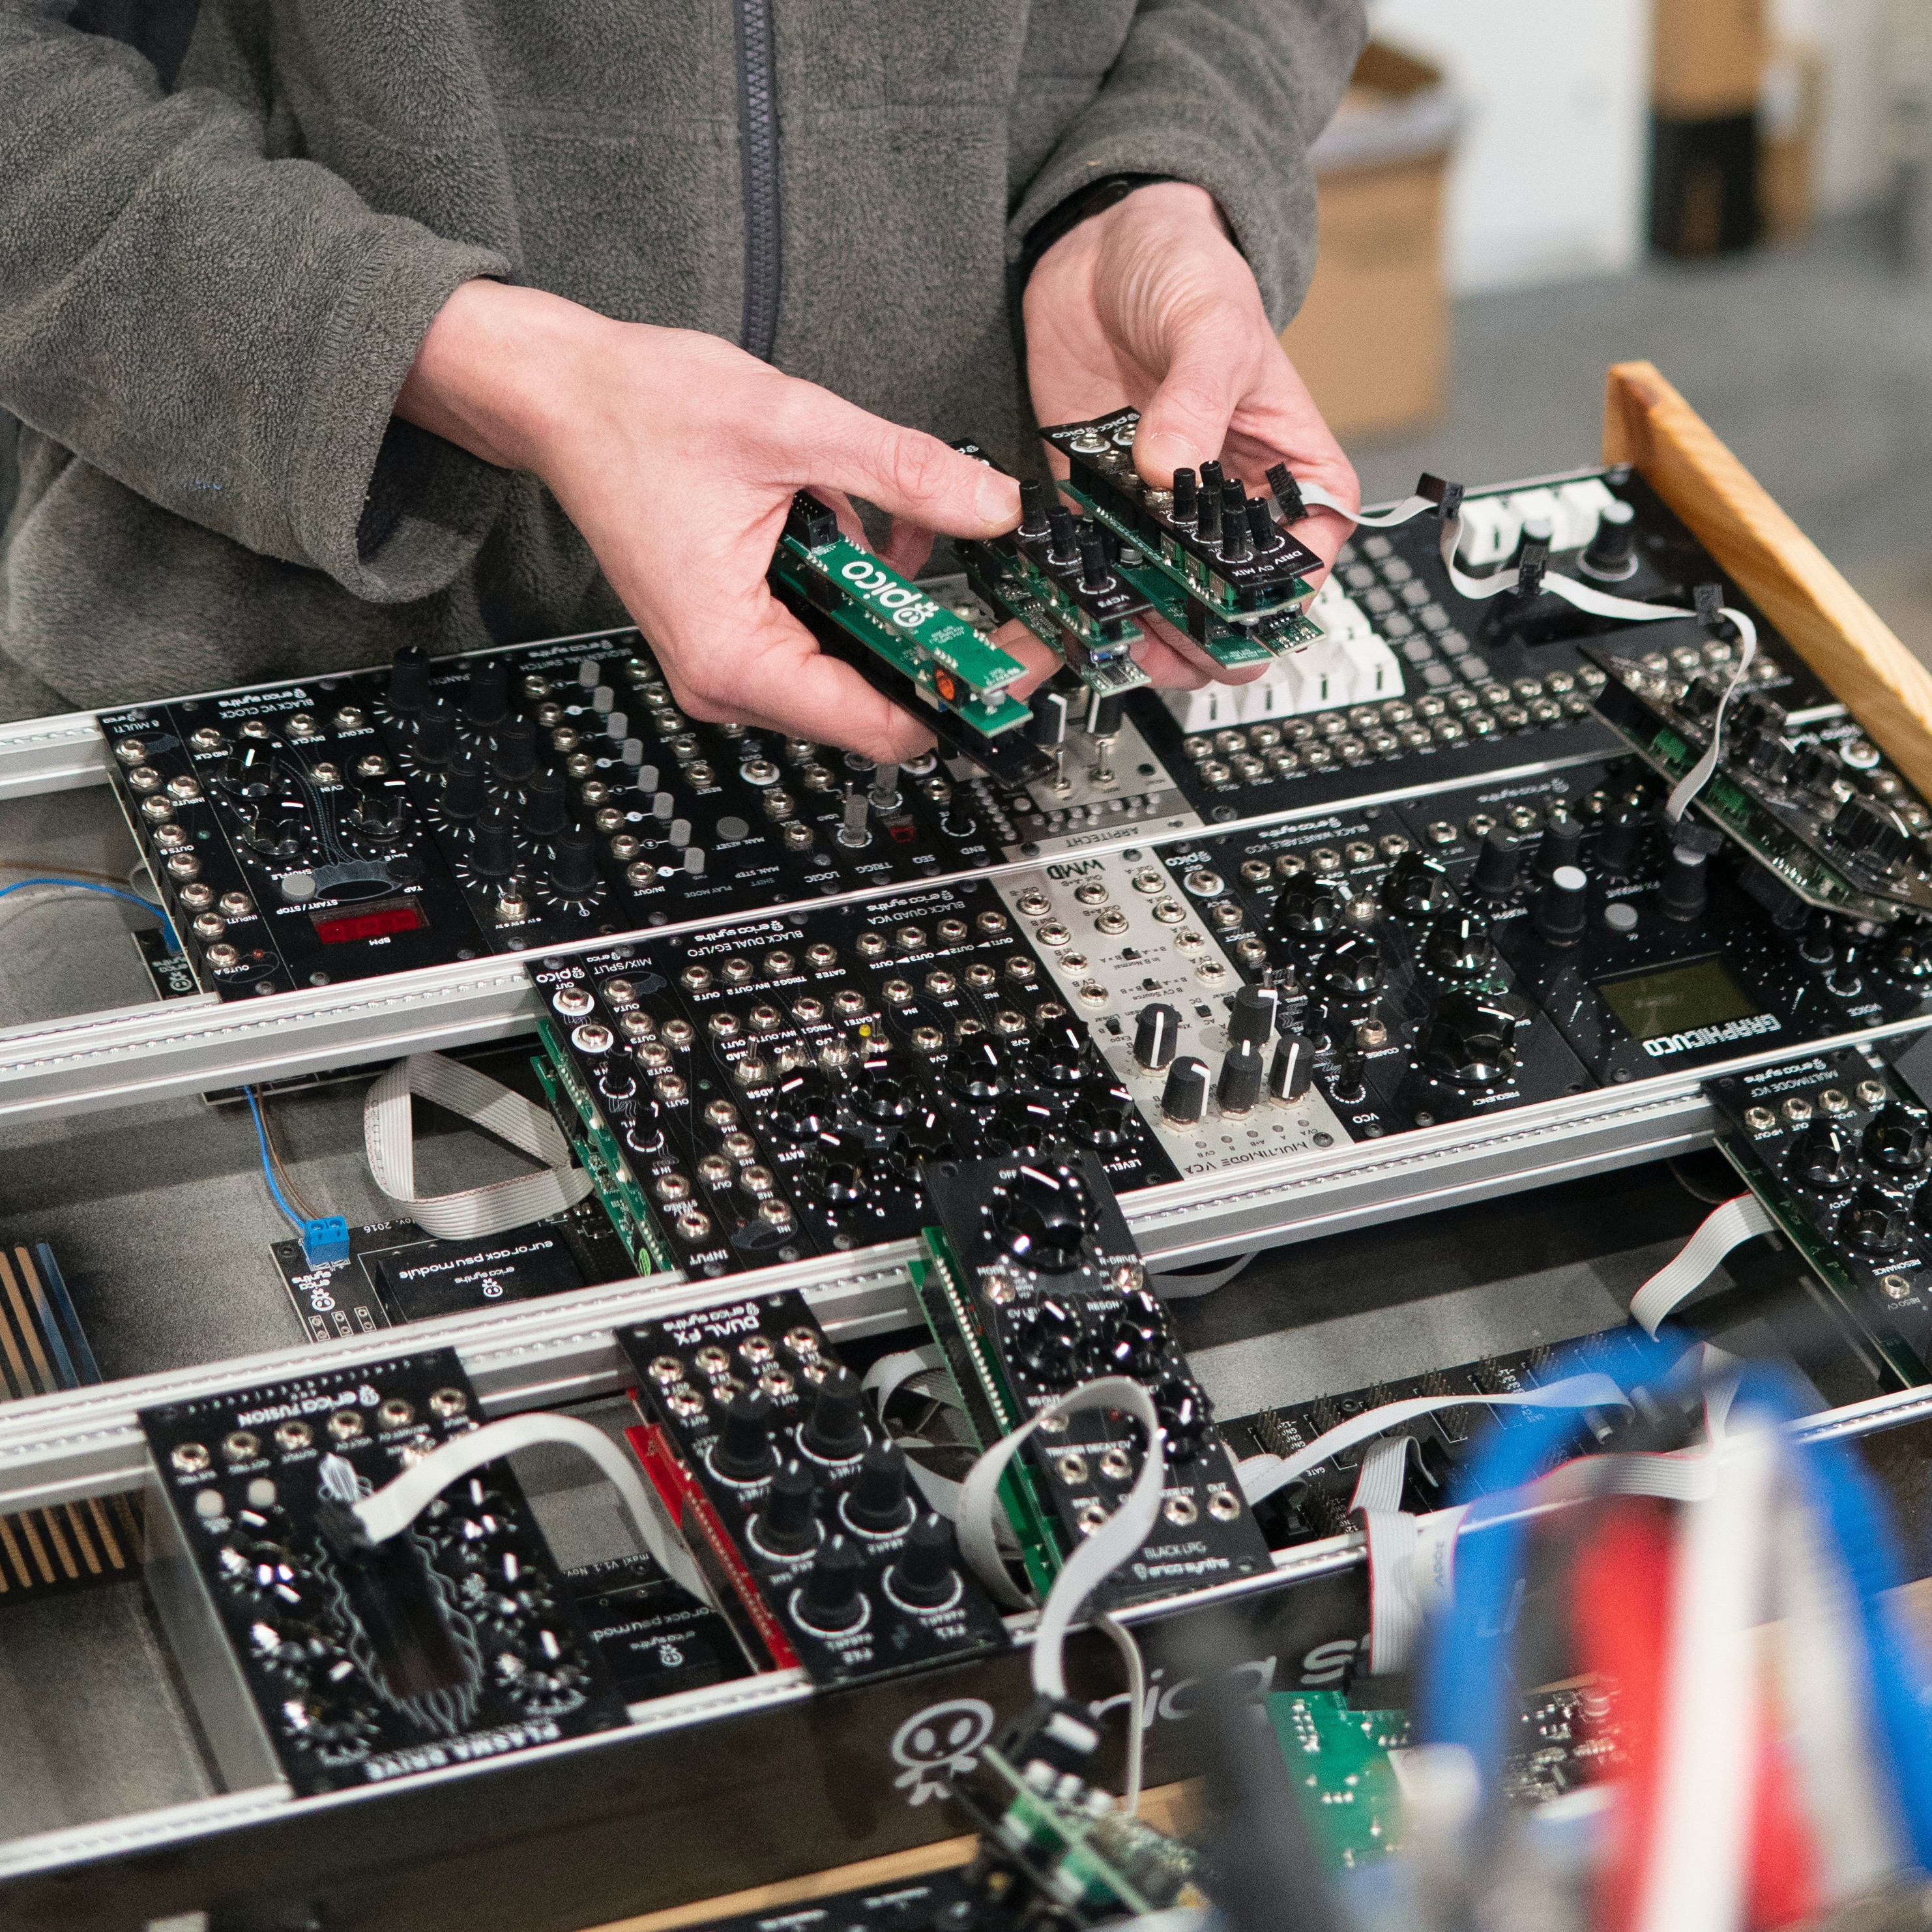
\includegraphics[width=0.8\linewidth]{modular-synth.jpg}
    \caption{Syntezator modułowy.}
  \end{figure}
  \end{multicols}
\end{frame}

\begin{frame}
  \frametitle{Jak algorytmicznie wyworzyć układ DSP generujący zadany dźwięk?}

  \begin{figure}
    \centering
    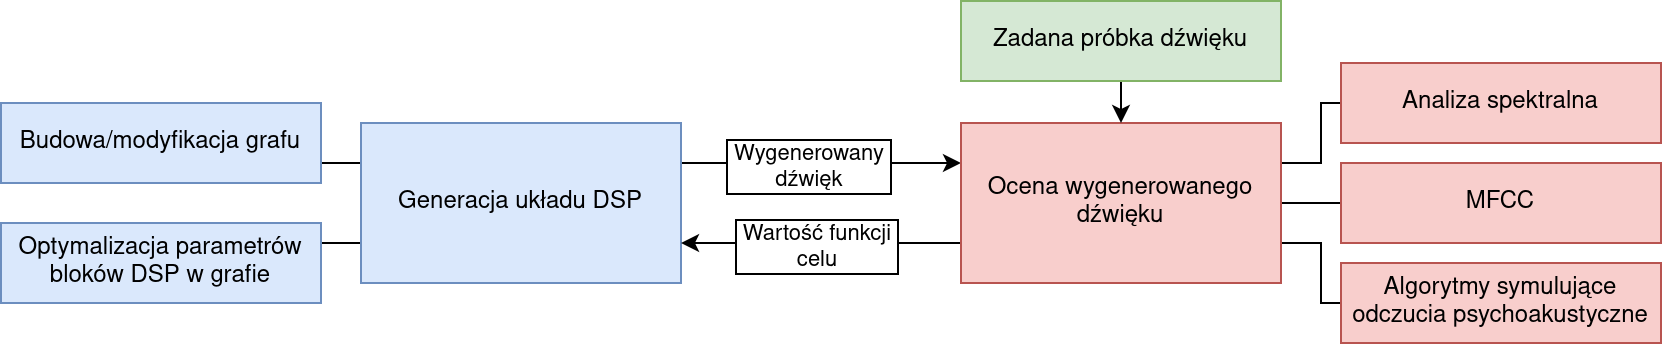
\includegraphics[width=1.0\linewidth]{algorithm-diagram.png}
    \caption{Diagram algorytmu realizowanego w ramach pracy.}
  \end{figure}
\end{frame}

\section{Bibliografia}

\begin{frame}
  \begin{thebibliography}{99} % Beamer does not support BibTeX so references must be nserted manually as below

  \bibitem[Zhang, 2023]{language_models_drummers} Zhang, Li and Callison-Burch, Chris
  \newblock Language Models are Drummers: Drum Composition with Natural Language Pre-Training
  \newblock \url{https://arxiv.org/abs/2301.01162}

  \bibitem[Forsgren, 2023]{riffusion} Forsgren, Seth* and Martiros, Hayk*
  \newblock Riffusion - Stable diffusion for real-time music generation
  \newblock \url{https://riffusion.com/about},

  \bibitem[Engel, 2017]{nsynth} Jesse and Resnick, Cinjon and Roberts, Adam and Dieleman, Sander and Eck, Douglas and Simonyan, Karen and Norouzi, Mohammad
  \newblock Neural Audio Synthesis of Musical Notes with WaveNet Autoencoders
  \newblock \url{https://arxiv.org/abs/1704.01279}

  \bibitem[Korg, 2019]{minilogue_diagram} Korg Inc,
  \newblock Korg Minilogue xd User Manual,
  \newblock \url{https://www.korg.com/us/support/download/manual/0/811/4277/}

  \end{thebibliography}
\end{frame}

% \begin{frame}
%   \begin{thebibliography}{99} % Beamer does not support BibTeX so references must be nserted manually as below
%   \bibitem[Shetty, 2017]{gartner2} Sony Shetty (2017)
%   \newblock How to Start an IT Monitoring Initiative
%   \newblock \emph{Gartner Insights}
%   \newblock \url{https://www.gartner.com/smarterwithgartner/how-to-start-an-it-monitoring-initiative}

%   \end{thebibliography}
% \end{frame}

\end{document}

